\section{eo\-FDCStat$<$ EOT $>$ Class Template Reference}
\label{classeo_f_d_c_stat}\index{eoFDCStat@{eoFDCStat}}
The FDC computation - stores the values into eo\-Value\-Param$<$EOT,double$>$ so they can be snapshot by some eo\-Gnuplot\-Snapshot ...  


{\tt \#include $<$eo\-FDCStat.h$>$}

Inheritance diagram for eo\-FDCStat$<$ EOT $>$::\begin{figure}[H]
\begin{center}
\leavevmode
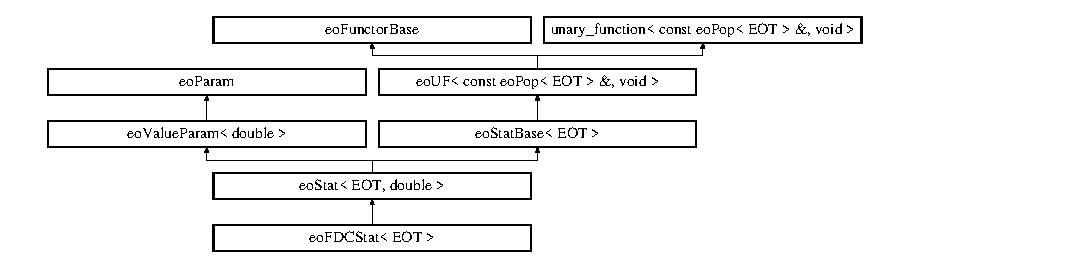
\includegraphics[height=3.15315cm]{classeo_f_d_c_stat}
\end{center}
\end{figure}
\subsection*{Public Member Functions}
\begin{CompactItemize}
\item 
{\bf eo\-FDCStat} ({\bf eo\-Distance}$<$ {\bf EOT} $>$ \&\_\-dist, std::string \_\-description=\char`\"{}FDC\char`\"{})\label{classeo_f_d_c_stat_a0}

\begin{CompactList}\small\item\em Ctor without the optimum. \item\end{CompactList}\item 
{\bf eo\-FDCStat} ({\bf eo\-Distance}$<$ {\bf EOT} $>$ \&\_\-dist, {\bf EOT} \&\_\-the\-Best, std::string \_\-description=\char`\"{}FDC\char`\"{})\label{classeo_f_d_c_stat_a1}

\begin{CompactList}\small\item\em Ctor with the optimum. \item\end{CompactList}\item 
virtual void {\bf operator()} (const {\bf eo\-Pop}$<$ {\bf EOT} $>$ \&\_\-pop)\label{classeo_f_d_c_stat_a2}

\begin{CompactList}\small\item\em Compute the FDC - either from best in pop, or from absolute best if it was passed in the constructor. \item\end{CompactList}\item 
const {\bf eo\-Value\-Param}$<$ std::vector$<$ double $>$ $>$ \& {\bf the\-Dist} ()\label{classeo_f_d_c_stat_a3}

\begin{CompactList}\small\item\em accessors to the private {\bf eo\-Value\-Param}{\rm (p.\,\pageref{classeo_value_param})}$<$std::vector$<$double$>$ $>$ \item\end{CompactList}\item 
const {\bf eo\-Value\-Param}$<$ std::vector$<$ double $>$ $>$ \& {\bf the\-Fit} ()\label{classeo_f_d_c_stat_a4}

\end{CompactItemize}
\subsection*{Private Attributes}
\begin{CompactItemize}
\item 
{\bf eo\-Distance}$<$ {\bf EOT} $>$ \& {\bf dist}\label{classeo_f_d_c_stat_r0}

\item 
{\bf EOT} {\bf the\-Best}\label{classeo_f_d_c_stat_r1}

\item 
bool {\bf bool\-Opt}\label{classeo_f_d_c_stat_r2}

\item 
{\bf eo\-Value\-Param}$<$ std::vector$<$ double $>$ $>$ {\bf dist\-To\-Best}\label{classeo_f_d_c_stat_r3}

\item 
{\bf eo\-Value\-Param}$<$ std::vector$<$ double $>$ $>$ {\bf fitnesses}\label{classeo_f_d_c_stat_r4}

\end{CompactItemize}


\subsection{Detailed Description}
\subsubsection*{template$<$class EOT$>$ class eo\-FDCStat$<$ EOT $>$}

The FDC computation - stores the values into eo\-Value\-Param$<$EOT,double$>$ so they can be snapshot by some eo\-Gnuplot\-Snapshot ... 



Definition at line 39 of file eo\-FDCStat.h.

The documentation for this class was generated from the following file:\begin{CompactItemize}
\item 
eo\-FDCStat.h\end{CompactItemize}
